\documentclass[12pt]{article}

% Review copy: one column, double spaced, numbered lines.
% The scientific content has been reorganized for a statistics/methods audience.
\usepackage[margin=1in]{geometry}
\usepackage{amsmath,amssymb,bm,amsthm}
\usepackage{graphicx}
\usepackage{booktabs,array,multirow}
\usepackage{setspace}
\usepackage{lineno}
\usepackage[numbers,sort&compress]{natbib}
\usepackage{url}
\usepackage{xcolor}
\usepackage[colorlinks=true,linkcolor=blue,citecolor=blue,urlcolor=blue]{hyperref}
\providecommand{\tightlist}{}
\setlength{\emergencystretch}{3em}

\newtheorem{proposition}{Proposition}
\newtheorem{corollary}{Corollary}
\newtheorem{lemma}{Lemma}
\theoremstyle{definition}
\newtheorem{definition}{Definition}
\theoremstyle{remark}
\newtheorem{remark}{Remark}

\newcommand{\dTV}{d_{\mathrm{TV}}}
\newcommand{\Neff}{N_{\mathrm{eff},p}}

\title{Null transport under temporal coarse-graining:\\ lumpability and surrogate inference for threshold-derived time series}
\author{Mauricio Herrera-Mar\'in\\[2pt]
\small Faculty of Engineering, Universidad del Desarrollo, Santiago, Chile\\
\small \texttt{mherrera@udd.cl}\quad ORCID: 0000-0002-9604-3077}
\date{}

\begin{document}
\doublespacing
\linenumbers
\maketitle

\begin{abstract}
Many environmental time-series analyses transform a native-resolution process into threshold-defined events and aggregated indices before imposing a resampling or surrogate null. We formulate the resulting problem as \emph{null transport}. A native randomization kernel $K_X$ and preprocessing map $\mathcal G$ admit an exact aggregate-space quotient null if and only if $K_X$ is strongly $\mathcal G$-lumpable: the pushed-forward law $\mathcal G_\#K_X(x,\cdot)$ must be constant over every fiber of $\mathcal G$. We give a quotient-kernel criterion, an unavoidable aggregate-only error bound when lumpability fails, and an exactly solvable example in which marginal-preserving spectral conditioning destroys lumpability after aggregation.

In a prespecified 13,500-trajectory benchmark, an annual marginal-and-spectrum IAAFT contract and a native-resolution constrained surrogate produced 1084 index-only rejections versus 16 native-only rejections. Concentrating a fixed expected annual event count raised index-only discordance from 4.4\% to 16.2\%; probability equalization reduced it from 15.9\% to 3.9\% in an independent experiment. Post hoc mechanism diagnostics show that the discrepancy is small for a continuous Gaussian annual mean, grows as the observable approaches a hard threshold count, and is accompanied by strong projected-null distortion. A within-fiber experiment held the complete event chronology and aggregate count sequence fixed yet changed the native pushed-forward null, providing direct numerical evidence against strong lumpability of the implemented contract.

A prospectively frozen application to 31 Chilean PM$_{2.5}$ monitoring stations (2018--2025) gave 29 index-only, zero native-only, and two joint rejections at the fixed $50\,\mu\mathrm{g\,m^{-3}}$ daily event threshold (region-level exact sign-flip $p=0.0039$). The index-null median Ferro--Segers center was 0.993 versus 0.557 for the native transported null. Equalizing monthly event probabilities reduced index-only decisions to five and reduced the null-center gap at all 31 stations. A prespecified null-width contraction prediction was not supported, showing that transport defects should be characterized through the full projected null distribution rather than variance alone. The inferential question is therefore not merely where a null is imposed, but whether that null can be transported through a lossy transformation and how any transport defect projects onto the chosen statistic.
\end{abstract}

\vspace{4pt}
\noindent\textbf{Keywords:} null transport; lumpability; surrogate data; coarse-graining; threshold exceedances; temporal aggregation; extremal clustering; air pollution

\clearpage
\section{Introduction}\label{sec:intro}

Environmental time series are often analyzed only after substantial deterministic preprocessing. Daily or monthly observations are thresholded into events, combined into annual counts or durations, detrended, and then supplied to a statistical test. Dry-month counts, frost days, heat-wave durations, low-flow spells, and many standard climate-extreme indices have this structure \cite{Sillmann2013,YangXu2017,BrunnerVoigt2024}. The transformation is scientifically meaningful, but it is also inferentially consequential: a hypothesis imposed on the derived index need not be the image of a hypothesis defined for the process that generated the index.

Surrogate-data methods make this issue especially transparent. A surrogate procedure defines a constrained null ensemble by preserving selected properties of the observed series and randomizing the remainder \cite{Theiler1992,SchreiberSchmitz1996,Schreiber1998,SchreiberSchmitz2000}. The preserved properties are therefore part of the null hypothesis itself. IAAFT surrogates, for example, preserve the empirical marginal distribution exactly and approximately preserve Fourier amplitudes \cite{SchreiberSchmitz1996}. The literature has long emphasized that surrogate algorithms must be checked against the null they are intended to represent, and that marginal and spectral agreement need not preserve higher-order or event-localization structure \cite{Kugiumtzis1999,Venema2006,Keylock2012}. Our question is different but complementary: what happens when nominally analogous constraints are imposed on opposite sides of a many-to-one transformation?

Temporal aggregation can change stochastic model form even for elementary linear processes \cite{StramWei1986}, and lossy transformations can create apparent dependence or obscure the distinction between genuine and spurious memory \cite{Maraun2004,Ohanissian2008}. A classical language for asking whether a stochastic mechanism survives state aggregation is \emph{lumpability}. For finite Markov chains, Kemeny and Snell gave a necessary and sufficient block-transition criterion; related work studies Markovian functions, exact and approximate aggregation, and conditions under which projected dynamics retain a closed description \cite{BurkeRosenblatt1958,KemenySnell1976,RogersPitman1981,Buchholz1994,Geiger2026}. We adapt that idea to a different object: the \emph{randomization kernel} defining a surrogate null on a trajectory space. We do not assume that the physical environmental process itself is a lumpable Markov chain.

Let $X$ denote a native-resolution trajectory, $\mathcal G$ a deterministic preprocessing map, and $K_X(x,dx^\star)$ the native randomization kernel. The pushed-forward law
\[
L_x=\mathcal G_\#K_X(x,\cdot)
\]
is the null distribution obtained by randomizing natively and then applying the same observation pipeline. An exact aggregate-space null depending only on $y=\mathcal G(x)$ exists if and only if $L_x$ is constant over each fiber $\mathcal G^{-1}(y)$. This is the kernel-lumpability condition developed below. It separates two questions that are otherwise easy to conflate: whether a unique quotient null exists after coarse-graining, and whether a chosen index-level surrogate is that quotient null.

Threshold-derived indices provide a useful controlled setting because their information loss can be described explicitly. If $F_m$ is the continuous marginal for calendar month $m$, the event $X_{y,m}<u_m$ is equivalent to $U_{y,m}<p_m$ for $U_{y,m}=F_m(X_{y,m})$ and $p_m=F_m(u_m)$. Conditional on the temporal copula, the entire indicator process therefore depends on the marginal/threshold construction through the vector $\mathbf p=(p_1,\ldots,p_{12})$. Seasonal concentration of $\mathbf p$ becomes a natural experimental coordinate, summarized here by the effective seasonal probability support
\[
\Neff=\frac{(\sum_m p_m)^2}{\sum_m p_m^2}.
\]

We combine theory, a prespecified synthetic benchmark, mechanism-localization controls, and a prospectively frozen environmental application. The confirmatory benchmark crosses three short-memory generator families, three persistence levels, five seasonal probability profiles, and 300 trajectories per cell. It compares an index-resolution IAAFT contract imposed after thresholding, annual aggregation, and detrending with a constrained monthly surrogate propagated through the identical transformation. An independent experiment directly equalizes monthly event probability. After those confirmatory analyses were completed, Gaussian oracle controls, a soft-to-hard threshold ablation, and a within-fiber perturbation were designed to localize the discrepancy. Finally, after the null-transport framework and synthetic mechanism results were available but before any application-level surrogate output was inspected, we froze a 31-station PM$_{2.5}$ cohort from Chile's National Air Quality Information System (SINCA) and a complete inferential protocol for daily-to-weekly threshold aggregation.

The results support five conclusions. First, null placement produced a highly asymmetric decision pattern in the confirmatory benchmark: 1084 trajectories rejected only under the index-level contract and 16 only under the native contract. Second, seasonal event-probability concentration amplified that discrepancy, while probability equalization removed most of the concentration-associated component. Third, Gaussian controls show that the large discrepancy is not a generic finite-sample behavior of annual IAAFT: it is small for a continuous linearly aggregated Gaussian observable and becomes pronounced as the observation approaches a hard threshold count. Fourth, a within-fiber experiment shows that two native trajectories with exactly the same complete threshold-indicator chronology and annual count sequence can induce substantially different pushed-forward native nulls because the native contract still uses hidden monthly amplitude organization. Fifth, the prospectively frozen SINCA application reproduces the inferential separation in observational data: at the fixed 24-hour PM$_{2.5}$ standard level, 29 of 31 stations rejected only under the weekly index-level null and none rejected only under the native transported null; seasonally equalizing event probability reduced the index-only count to five. The central issue is therefore not simply \emph{where} a null is imposed, but whether the information needed to define that null survives the transformation and how any resulting transport defect projects onto the statistic used for inference.

\section{Null transport and analytical framework}\label{sec:theory}

\subsection{Native and index-level inferential paths}\label{sec:paths}

Let $X=\{X_{y,m}\}$ be a monthly process. The threshold-and-aggregation operator $\mathcal O$ first forms
\[
I_{y,m}=\mathbf 1\{X_{y,m}<u_m\}
\]
and then the annual count
\[
C_y=\sum_{m=1}^{12}I_{y,m}.
\]
A fixed cubic-detrending rule $D$ produces $Z=D(C)$, and the full preprocessing map is $\mathcal P=D\circ\mathcal O$.

The native and index-resolution paths are
\[
X\xrightarrow{K_X}X^\star\xrightarrow{\mathcal P}Z^\star_{\rm native},
\qquad
X\xrightarrow{\mathcal P}Z\xrightarrow{K_Y}Z^\star_{\rm index}.
\]
At the level of distributions, the first path induces $\mathcal P_\#K_X(x,\cdot)$, whereas the second uses the selected aggregate-space kernel $K_Y(\mathcal P x,\cdot)$. Equality is not automatic; it is a structural property of the pair $(K_X,\mathcal P)$ and of the chosen $K_Y$.

\subsection{Kernel lumpability and quotient nulls}\label{sec:lumpability}

Let $(\mathsf X,\mathcal A)$ be a native trajectory space, $(\mathsf Y,\mathcal B)$ a derived-data space, and $\mathcal G:\mathsf X\to\mathsf Y$ a measurable deterministic map. Let $K_X$ be a Markov kernel on $\mathsf X$. For observed $x$, define the transported native null
\begin{equation}
L_x(B)=K_X\!\left(x,\mathcal G^{-1}(B)\right),\qquad B\in\mathcal B.
\label{eq:transport}
\end{equation}
Thus $L_x=\mathcal G_\#K_X(x,\cdot)$.

\begin{definition}[Strong $\mathcal G$-lumpability of a randomization kernel]
$K_X$ is strongly $\mathcal G$-lumpable if
\begin{equation}
L_x=L_{x'}\quad\text{whenever}\quad \mathcal G(x)=\mathcal G(x').
\label{eq:lumpability}
\end{equation}
Equivalently, the transported native null depends on $x$ only through the derived observation $y=\mathcal G(x)$.
\end{definition}

This definition applies the classical lumpability idea to a one-step randomization kernel on trajectories rather than to the physical time evolution. In finite state spaces it reduces to the familiar requirement that all microstates in a block have the same total transition probability into every target block \cite{KemenySnell1976,Buchholz1994}.

\begin{proposition}[Quotient-null criterion]\label{prop:quotient}
Equip $\mathsf Y=\mathcal G(\mathsf X)$ with the quotient sigma-algebra induced by $\mathcal G$. The following are equivalent:
\begin{enumerate}
\item $K_X$ is strongly $\mathcal G$-lumpable;
\item there exists a Markov kernel $\bar K_Y$ on $\mathsf Y$ such that
\begin{equation}
\mathcal G_\#K_X(x,\cdot)=\bar K_Y(\mathcal Gx,\cdot)
\qquad\text{for every }x\in\mathsf X.
\label{eq:quotient}
\end{equation}
\end{enumerate}
On $\mathcal G(\mathsf X)$ the kernel $\bar K_Y$ is unique.
\end{proposition}

\begin{proof}
If \eqref{eq:quotient} holds and $\mathcal Gx=\mathcal Gx'$, both transported laws equal $\bar K_Y(\mathcal Gx,\cdot)$, proving lumpability. Conversely, if \eqref{eq:lumpability} holds, define $\bar K_Y(y,B)=L_x(B)$ for any $x\in\mathcal G^{-1}(\{y\})$. Lumpability makes the definition independent of the representative, and measurability follows from the quotient sigma-algebra. Uniqueness on the image of $\mathcal G$ is immediate.
\end{proof}

Proposition~\ref{prop:quotient} distinguishes an \emph{existence problem} from a \emph{surrogate-substitution problem}. Even when a quotient null $\bar K_Y$ exists, a selected index-level kernel $K_Y$ need not equal it. Conversely, if strong lumpability fails, no single aggregate-only kernel can reproduce all native transported nulls over a fiber.

\subsection{Transport defects and projection to a test statistic}\label{sec:defects}

For $y\in\mathsf Y$, define the fiber $\mathcal F_y=\{x:\mathcal Gx=y\}$ and its total-variation transport diameter
\begin{equation}
\Delta_L(y)=\sup_{x,x'\in\mathcal F_y}\dTV(L_x,L_{x'}).
\label{eq:DeltaL}
\end{equation}
Then $\Delta_L(y)=0$ for every $y$ if and only if $K_X$ is strongly $\mathcal G$-lumpable.

\begin{proposition}[Unavoidable error of an aggregate-only null]\label{prop:halfdiam}
For any kernel $Q_Y(y,\cdot)$ that has access only to the derived observation $y$,
\begin{equation}
\sup_{x\in\mathcal F_y}\dTV\!\left(L_x,Q_Y(y,\cdot)\right)
\ge \frac12\Delta_L(y).
\label{eq:halfdiam}
\end{equation}
Thus, if $\Delta_L(y)>0$, no aggregate-only null can uniformly reproduce the native transported null over that fiber.
\end{proposition}

\begin{proof}
For any $x,x'\in\mathcal F_y$, the triangle inequality gives
\[
\dTV(L_x,L_{x'})\le \dTV(L_x,Q_Y)+\dTV(Q_Y,L_{x'}).
\]
At least one term on the right is at least half the left-hand side. Taking the supremum over $x,x'$ yields \eqref{eq:halfdiam}.
\end{proof}

The kernel-level defect need not be visible to every statistic. If $T:\mathsf Y\to\mathsf Z$ is measurable, then the data-processing inequality gives
\begin{equation}
\dTV(T_\#L_x,T_\#L_{x'})\le \dTV(L_x,L_{x'}).
\label{eq:dataprocessing}
\end{equation}
For a rejection set $R\subseteq\mathsf Z$,
\begin{equation}
\left|L_x\{T\in R\}-L_{x'}\{T\in R\}\right|
\le \dTV(T_\#L_x,T_\#L_{x'}).
\label{eq:decisionbound}
\end{equation}

\begin{corollary}[Projected witness of non-lumpability]\label{cor:projected}
If $\mathcal Gx=\mathcal Gx'$ and there exists a measurable statistic $T$ such that $T_\#L_x\neq T_\#L_{x'}$, then $K_X$ is not strongly $\mathcal G$-lumpable.
\end{corollary}

\begin{proof}
Strong $\mathcal G$-lumpability would imply $L_x=L_{x'}$ and therefore equality after every measurable pushforward $T$. The contrapositive gives the result.
\end{proof}

We therefore distinguish a kernel-level transport defect, a statistic-projected defect, and decision discordance. Large kernel differences may be attenuated by a particular statistic, while a difference in the statistic-level null is direct evidence that the underlying transported kernels cannot be identical. Corollary~\ref{cor:projected} is the formal basis for the within-fiber diagnostic in Section~\ref{sec:fibermethods}.

\subsection{Model-dependent transport when strong lumpability fails}\label{sec:modeltransport}

Failure of strong lumpability does not prevent all aggregate-space inference; it changes what must be specified. Let $P_0$ be a benchmark model on $\mathsf X$ with regular conditional distribution $\mu_y(dx)=P_0(dx\mid\mathcal G(X)=y)$. Define
\begin{equation}
\bar K_{P_0}(y,B)=\int_{\mathcal F_y}L_x(B)\,\mu_y(dx).
\label{eq:modeltransport}
\end{equation}
If $X\sim P_0$ and $X^\star\mid X\sim K_X(X,\cdot)$, then
\begin{equation}
\Pr\{\mathcal G(X^\star)\in B\mid\mathcal G(X)=y\}=\bar K_{P_0}(y,B).
\label{eq:conditionaltransport}
\end{equation}
Under strong lumpability, \eqref{eq:modeltransport} reduces to the unique quotient kernel for every $P_0$. Otherwise, the transported null depends on how unresolved native microstates are distributed within the observed fiber. In that sense, the aggregate alone does not identify the native inferential contract.

\subsection{An exactly solvable spectral-conditioning counterexample}\label{sec:counterexample}

The following finite example isolates a mechanism relevant to marginal-and-spectrum surrogates. It is not an analytical representation of IAAFT; rather, it shows that exact marginal preservation combined with microstate spectral conditioning can destroy lumpability after aggregation.

Let
\[
\Omega=\left\{z\in\{0,1\}^{4}:\sum_{t=1}^{4}z_t=2\right\},
\]
and define the two-block aggregation
\begin{equation}
\mathcal O(z)=(z_1+z_2,z_3+z_4).
\label{eq:toyO}
\end{equation}
With $\bar z=1/2$, define the circular lag-one score
\begin{equation}
R(z)=\sum_{t=1}^{4}(z_t-\bar z)(z_{t+1}-\bar z),\qquad z_5=z_1.
\label{eq:toyR}
\end{equation}
By the discrete Wiener--Khinchin relation, $R$ is a linear functional of Fourier power. For $\tau\ge0$, define the marginal-preserving spectral-tilted kernel
\begin{equation}
K_\tau(x,z)=
\frac{\exp\{-\tau[R(z)-R(x)]^2\}}
{\sum_{w\in\Omega}\exp\{-\tau[R(w)-R(x)]^2\}},
\qquad z\in\Omega.
\label{eq:toykernel}
\end{equation}
At $\tau=0$ this is uniform over all permutations; increasing $\tau$ favors permutations whose spectral score resembles that of the observed microstate.

\begin{proposition}[Spectral conditioning can destroy lumpability]\label{prop:toy}
For the map \eqref{eq:toyO}, $K_0$ is strongly $\mathcal O$-lumpable, whereas $K_\tau$ is not strongly $\mathcal O$-lumpable for any $\tau>0$. In particular, for
\[
x=(0,1,1,0),\qquad x'=(1,0,1,0),
\]
we have $\mathcal O(x)=\mathcal O(x')=(1,1)$ but $R(x)=0$ and $R(x')=-1$. Writing $q=e^{-\tau}$,
\begin{equation}
\dTV\!\left(\mathcal O_\#K_\tau(x,\cdot),\mathcal O_\#K_\tau(x',\cdot)\right)
=
\frac{1-q^2}{2q^2+5q+2}>0
\quad(\tau>0).
\label{eq:toyTV}
\end{equation}
The distance tends to $1/2$ as $\tau\to\infty$.
\end{proposition}

\begin{proof}
Among the six states in $\Omega$, four have $R=0$ and two have $R=-1$. The possible block counts are $(2,0)$, $(1,1)$, and $(0,2)$. For $x$ the transported distribution is
\[
L_x=\frac{1}{4+2q}(1,2+2q,1),
\]
whereas for $x'$ it is
\[
L_{x'}=\frac{1}{2+4q}(q,2+2q,q).
\]
They coincide only at $q=1$. Direct calculation yields \eqref{eq:toyTV}.
\end{proof}

For $T_{\rm diff}(y_1,y_2)=(y_2-y_1)^2$, the total-variation distance between the two induced statistic distributions equals \eqref{eq:toyTV}; this statistic retains the entire transport defect in the example. Proposition~\ref{prop:halfdiam} then implies that every aggregate-only null on the fiber $\mathcal O^{-1}(1,1)$ incurs worst-case total-variation error at least half of \eqref{eq:toyTV}. The obstruction is therefore not merely that a particular aggregate surrogate is inconvenient: once the native kernel uses a spectral feature erased by $\mathcal O$, the aggregate cannot uniquely encode that contract.

\subsection{Threshold--copula reduction}\label{sec:copula}

\begin{lemma}[Threshold--copula reduction]\label{lem:copula}
Let $X_{y,m}$ have continuous, strictly increasing month-specific marginal distribution functions $F_m$. Define
\[
U_{y,m}=F_m(X_{y,m}),\qquad p_m=F_m(u_m).
\]
Then
\[
\mathbf 1\{X_{y,m}<u_m\}=\mathbf 1\{U_{y,m}<p_m\}
\quad\text{almost surely}.
\]
Hence the finite-dimensional distributions of the complete threshold-indicator process are determined by the finite-dimensional temporal copula of $U$ and the threshold-probability vector $\mathbf p=(p_1,\ldots,p_b)$.
\end{lemma}

\begin{proof}
Strict monotonicity gives $X_{y,m}<u_m$ if and only if $F_m(X_{y,m})<F_m(u_m)$. Every finite-dimensional probability for the indicator process is therefore a copula probability over a rectangle whose boundaries are the relevant $p_m$.
\end{proof}

The lemma separates a dependence coordinate, carried by the temporal copula, from a seasonal event-geometry coordinate, carried by $\mathbf p$. We summarize the latter by
\begin{equation}
\Neff=\frac{(\sum_{m=1}^{b}p_m)^2}{\sum_{m=1}^{b}p_m^2}.
\label{eq:neff}
\end{equation}
For fixed $K=\sum p_m$, Cauchy--Schwarz gives $\Neff\le b$, with equality if and only if $p_1=\cdots=p_b=K/b$. We use $\Neff$ descriptively rather than as a universal reliability threshold.

\subsection{Exact covariance of Gaussian threshold counts}\label{sec:gausscov}

The Gaussian branch permits an exact second-order calculation that makes explicit how $\mathbf p$ and native dependence are transformed by thresholding and aggregation.

\begin{proposition}[Gaussian threshold-count covariance]\label{prop:gausscov}
Let $\{X_t\}$ be a stationary standard Gaussian AR(1) process with $\operatorname{Corr}(X_t,X_{t+h})=\phi^{|h|}$, $|\phi|<1$. Let month $m$ use threshold $u_m=\Phi^{-1}(p_m)$ and define
\[
C_y=\sum_{m=1}^{12}\mathbf 1\{X_{12(y-1)+m}<u_m\}.
\]
For integer $k\ge0$,
\begin{equation}
\gamma_C(k)
=
\sum_{m=1}^{12}\sum_{n=1}^{12}
\left[
\Phi_2\!\left(u_m,u_n;\phi^{|12k+n-m|}\right)-p_mp_n
\right],
\label{eq:gausscov}
\end{equation}
where $\Phi_2(a,b;\rho)$ is the standard bivariate normal distribution function with correlation $\rho$ (with the degenerate $\rho=1$ case understood by continuity). Consequently, the population spectrum of the annual count is
\begin{equation}
f_C(\omega)=\frac{1}{2\pi}\left[\gamma_C(0)+2\sum_{k=1}^{\infty}\gamma_C(k)\cos(k\omega)\right].
\label{eq:gaussspectrum}
\end{equation}
\end{proposition}

\begin{proof}
Write $I_{y,m}=\mathbf 1\{X_{12(y-1)+m}<u_m\}$. For any $(y,m)$ and $(y+k,n)$, the underlying pair is bivariate normal with correlation $\phi^{|12k+n-m|}$, so
\[
\operatorname{Cov}(I_{y,m},I_{y+k,n})
=\Phi_2(u_m,u_n;\phi^{|12k+n-m|})-p_mp_n.
\]
Summing over $m,n$ yields \eqref{eq:gausscov}. Because the Gaussian indicator covariance decays geometrically with the underlying AR(1) correlation, $\sum_k|\gamma_C(k)|<\infty$, so the Fourier series \eqref{eq:gaussspectrum} is well defined.
\end{proof}

Equation~\eqref{eq:gausscov} is useful for interpretation even though the main surrogate algorithms condition on sample quantities rather than on the population spectrum. It shows exactly what second-order information the hard threshold-and-count map induces from a linear Gaussian native process; it also supplies a population benchmark against which sample-spectrum constraints can be diagnosed.

\section{Methods}\label{sec:methods}

\subsection{Short-memory generators and seasonal event geometry}\label{sec:generators}

The confirmatory benchmark used three monthly short-memory generator families, each with $\phi\in\{0.2,0.5,0.8\}$. The first was a stationary Gaussian AR(1),
\[
X_t=\phi X_{t-1}+\sqrt{1-\phi^2}\,\varepsilon_t,
\qquad \varepsilon_t\sim N(0,1).
\]
The second was a Gaussian AR(1) with periodic innovation scale,
\[
X_t=\phi X_{t-1}+\sigma_{m(t)}\varepsilon_t,
\qquad
\sigma_m=\exp\!\left[0.65\cos\!\left(\frac{2\pi(m-1)}{12}\right)\right].
\]
Calendar-month state variances were obtained from the periodic variance recursion. The third used standardized Student-$t$ innovations with $\nu=5$,
\[
X_t=\phi X_{t-1}+\eta_t,
\qquad
\eta_t=\sqrt{\frac{\nu-2}{\nu}}\,T_\nu,
\]
with thresholds calibrated from fixed 300,000-point reference simulations. Each trajectory contained 252 simulated years; the primary fixed-phase analysis used the first 251 complete 12-month windows.

Event probabilities were
\begin{equation}
p_m(\lambda)=\operatorname{logit}^{-1}\!\left[a_\lambda+\lambda\cos\!\left(\frac{2\pi(m-8)}{12}\right)\right],
\label{eq:profile}
\end{equation}
where $a_\lambda$ was chosen so that $\sum_m p_m=3$. The prespecified grid $\lambda\in\{0,0.5,1,2,4\}$ corresponds to $\Neff\approx12.00,11.24,9.63,6.98,4.96$. Thresholds were chosen within each generator family so that all families realized the same $\mathbf p$ profile.

\subsection{Annual observable, detrending, and test statistic}\label{sec:observable}

The primary annual observable was
\[
C_y=\sum_{m=1}^{12}\mathbf 1\{X_{y,m}<u_m\}.
\]
Each annual series was detrended by ordinary least squares against a cubic polynomial in $t_y\in[-1,1]$,
\[
Z_y=D(C)_y=C_y-\widehat g_3(t_y).
\]
The same rule was fitted separately to every observed or surrogate annual series.

Extremal clustering was summarized by the intervals estimator of Ferro and Segers \cite{FerroSegers2003}. Let $u_q=Q_{0.90}(Z)$ and let $s_1<\cdots<s_N$ index values above $u_q$. With $T_i=s_{i+1}-s_i$, $S_i=T_i-1$, and $n_T=N-1$,
\[
\widehat\theta_{\rm raw}=
\begin{cases}
\dfrac{2(\sum_iT_i)^2}{n_T\sum_iT_i^2},&\max_iT_i\le2,\\[1.4ex]
\dfrac{2(\sum_iS_i)^2}{n_T\sum_iS_i(S_i-1)},&\max_iT_i>2.
\end{cases}
\]
Nonpositive denominators were assigned one, and confirmatory tests used $\widehat\theta=\operatorname{clip}(\widehat\theta_{\rm raw},0,1)$. Smaller values indicate stronger clustering.

\subsection{Index and native surrogate contracts}\label{sec:contracts}

The index-resolution contract was IAAFT applied to the cubic-detrended annual series $Z$. Each surrogate was initialized by a random permutation, iteratively projected onto the observed centered Fourier amplitudes, inverse transformed, and rank-remapped to the exact sorted values of $Z$. At most 30 iterations were used. The normalized spectral error was
\[
E_{\rm spec}=
\frac{\operatorname{mean}(|\widehat Z^\star|-|\widehat Z|)^2}
{\operatorname{mean}|\widehat Z|^2+10^{-15}}.
\]
Thus the annual contract preserves the empirical marginal exactly and approximately preserves the sample Fourier-amplitude spectrum.

The native contract acted on the monthly process before thresholding. Calendar-month means and standard deviations were used to standardize the observed monthly sequence. The target Fourier amplitudes were those of the standardized monthly record. Surrogates were initialized by permuting exact observed values within calendar month, projected onto the target monthly Fourier amplitudes, inverse transformed, and then rank-remapped within each calendar-month group to its exact observed value multiset. The procedure used at most 12 iterations. Afterward the fixed thresholds, annual count operator, detrending, and $\widehat\theta$ calculation were applied. A prespecified robustness contract used calendar month $\times$ 50-year blocks instead of full-record calendar-month groups.

For either contract, the lower-tail Monte Carlo p-value was
\[
p=\frac{1+\#\{\widehat\theta_b^\star\le\widehat\theta_{\rm obs}\}}{B+1},
\]
with strict rejection at $p<0.05$. With $B=249$, the attainable rejection probability under exchangeability is $12/250=0.048$. Define $A=\mathbf 1\{p_{\rm index}<0.05\}$ and $N=\mathbf 1\{p_{\rm native}<0.05\}$. The primary paired outcome is $A(1-N)$, termed \emph{index-only discordance}; the reverse event is $N(1-A)$.

\subsection{Prespecified confirmatory experiments}\label{sec:confirmatory}

The primary benchmark crossed three generator families, three $\phi$ values, five $\lambda$ values, and 300 independent trajectories per cell, for 13,500 trajectories. Each native and index test used $B=249$. The primary comparison was paired index-only versus native-only discordance, and the prespecified concentration contrast compared $\lambda=4$ with $\lambda=0$. Additional prespecified analyses included 50-year native grouping, the maximum within-year run as a secondary observable, and a complete 12-phase aggregation audit. The grouping result is summarized in the Supplement; the complete archived robustness outputs are retained in the confirmatory reproducibility package.

A separate independent probability-equalization cohort comprised 1350 trajectories (three generator families, three $\phi$ values, 150 replicates per cell; $B=149$). On each generating trajectory we compared the concentrated $\lambda=4$ profile, an oracle uniform profile $p_m=0.25$, and month-specific 25th-percentile thresholds estimated from independent 15-, 30-, and 60-year reference series. The concentrated-versus-oracle comparison was primary; the 30-year reference was the prespecified finite-calibration analysis.

A prespecified eight-unit sensitivity experiment assessed the ability of the native-resolution gate to detect two injected alternatives while preserving calendar-month value multisets and threshold-event counts: persistent-regime alignment and history feedback. It used 150 cohorts per design point and $B=500$ per unit. Full details are given in the Supplement.

\subsection{Gaussian oracle and operator-ablation diagnostics}\label{sec:ablationmethods}

After the confirmatory benchmark, mechanism-localization analyses were designed to distinguish generic finite-sample IAAFT behavior from an interaction with the observation operator. These analyses are diagnostic, not part of the original confirmatory protocol.

We used the stationary Gaussian AR(1) branch with $\phi\in\{0.2,0.5,0.8\}$, 100 independent trajectories per $\phi$, and $B=249$. For each observed trajectory, three null ensembles were compared: (i) a \emph{generative oracle} consisting of independent draws from the known AR(1) generator; (ii) the native constrained surrogate described above, followed by the chosen operator; and (iii) annual IAAFT applied after the operator. The oracle is available only because the diagnostic generator is known.

The continuous control was the annual mean, evaluated both before and after cubic detrending. To approach the hard count continuously, we defined
\begin{equation}
S_y(\tau)=\sum_{m=1}^{12}
\operatorname{logit}^{-1}\!\left(\frac{u_m-X_{y,m}}{\tau}\right),\qquad \tau>0,
\label{eq:soft}
\end{equation}
with $S_y(\tau)\to C_y$ as $\tau\downarrow0$. The $B=249$ operator-ablation grid used $\tau\in\{2,1,0.5,0.25,0.1\}$ and the hard-count limit, for both $\lambda=0$ and $\lambda=4$. The primary diagnostic summaries were rejection rates, paired index/native decisions, the null standard deviation of $\widehat\theta$, and spectral fidelity. A smaller independently seeded near-zero follow-up extended the path to $\tau=0.001$; its role was descriptive and it is reported in the Supplement.

\subsection{Within-fiber lumpability diagnostic}\label{sec:fibermethods}

To test the empirical implication of strong lumpability directly, we constructed pairs $x,\widetilde x$ satisfying $\mathcal O(x)=\mathcal O(\widetilde x)$ exactly. For each Gaussian AR(1) trajectory, $\widetilde x$ was formed by permuting exact amplitudes \emph{within each calendar-month $\times$ threshold-indicator class}. The construction therefore preserves the complete monthly event-indicator chronology, the entire annual count sequence, and every calendar-month empirical value multiset, mean, and variance. It generally changes the standardized monthly Fourier-amplitude target used by the native surrogate.

For each $x$, two independent native-surrogate ensembles were generated from $x$ to estimate Monte Carlo baseline variability, and a third was generated from $\widetilde x$. Each ensemble used $B=249$. We used 30 trajectories at each $\phi\in\{0.2,0.5,0.8\}$ for $\lambda=0$ and $\lambda=4$, giving 90 within-fiber pairs per seasonal profile. All construction checks were exact: there were no indicator mismatches, annual-count differences, or calendar-month multiset differences.

Pushed-forward distributions were compared for four projections: the Ferro--Segers statistic, annual lag-one correlation, the order-sensitive statistic
\[
T_{\rm diff}(C)=\frac{1}{n-1}\sum_{y=1}^{n-1}(C_{y+1}-C_y)^2,
\]
and the fraction of periodogram power in the lowest 10\% of nonzero frequencies after cubic detrending. Wasserstein distances were scaled by the pooled standard deviation of the two compared ensembles. For each pair, the within-fiber distance was compared with the distance between the two same-$x$ ensembles. Two-sample KS tests and one-sided sign tests were used only as diagnostic summaries, not as confirmatory claims about a pre-registered hypothesis.

\subsection{Prospectively frozen SINCA PM2.5 application}\label{sec:sincamethods}

Daily PM$_{2.5}$ observations were obtained from Chile's National Air Quality Information System (SINCA) through the AtmChile data interface \cite{Catalan2022,SINCA2026}. The analysis window was fixed at 1 January 2018 through 28 December 2025, yielding 417 complete Monday--Sunday weeks. Chilean D.S. No.~12/2011 sets the 24-hour primary PM$_{2.5}$ standard level at $50\,\mu\mathrm{g\,m^{-3}}$; legal exceedance of the standard is defined through the annual 98th percentile, so here $50$ is used as a scientifically and policy-relevant daily event threshold rather than treating every individual day above 50 as a statutory noncompliance event \cite{MMA2011}. The primary daily event was therefore
\[
I_{s,t}=\mathbf 1\{X_{s,t}>50\}.
\]

The station cohort was frozen before any SINCA surrogate result was computed. Eligibility required an unambiguous station identifier, at least 95\% daily coverage over the fixed window, at least 95\% of complete weeks with six or more observed days, at least 100 observed threshold events, no more than 0.1\% of values outside the diagnostic range $[0,500]$, and no gross recent scale-shift flag. These criteria yielded 31 stations across eight administrative regions. Their frozen monthly exceedance geometry spanned $\Neff=3.40$--$5.67$ (median 4.30). The exact station list and cohort hash are reported in the Supplement.

No stochastic event imputation was used. Let $\widehat p_{s,m}$ be the observed probability of $X_{s,t}>50$ in calendar month $m$. On observed days, $\widetilde I_{s,t}=I_{s,t}$; on missing days, $\widetilde I_{s,t}=\widehat p_{s,m(t)}$. The primary weekly burden was
\[
C_{s,w}=\sum_{t\in w}\widetilde I_{s,t}.
\]
Each weekly series was residualized against a cubic trend and the first three annual sine/cosine harmonics using the fixed design matrix
\[
1,t,t^2,t^3,\{\sin(2\pi k d/365.2425),\cos(2\pi k d/365.2425)\}_{k=1}^{3},
\]
where $d$ is the week midpoint in days. Ferro--Segers at $q=0.90$ was the primary statistic.

The native application contract acted on daily PM$_{2.5}$. Observed values were standardized by calendar month; missing positions were fixed at the month-specific standardized mean only for construction of the complete FFT sequence. The target Fourier amplitudes were those of this standardized daily sequence. Native surrogates iteratively projected onto those amplitudes and rank-remapped observed positions within calendar month to the exact observed raw-value multiset; the missing mask was fixed. The contract used 12 iterations and therefore preserved exact calendar-month observed values and exact observed calendar-month counts above the fixed threshold. Each native surrogate was then thresholded, aggregated weekly, residualized, and scored by the same statistic. The index-level contract applied 30-iteration IAAFT directly to the observed weekly residual series. Each station and contract used $B=499$, giving an attainable strict $p<0.05$ level of $24/500=0.048$.

Across stations, paired asymmetry was summarized by the counts of index-only and native-only decisions. Because stations within a region are dependent, the primary directional assessment was an exact sign-flip test over the eight represented regions, with each region contributing its signed difference between index-only and native-only counts. Benjamini--Yekutieli adjustment at $q=0.05$ was applied separately to native and index station-level $p$-values. A prespecified mechanistic summary tested whether seasonal concentration predicted null-width contraction through the Spearman association between frozen $\Neff$ and
\[
\log R_s=\log\left\{\frac{\operatorname{SD}(\widehat\theta^\star_{\rm index,s})}{\operatorname{SD}(\widehat\theta^\star_{\rm native,s})}\right\},
\]
with a 2000-resample region-cluster bootstrap interval.

A prospectively specified mechanism intervention replaced the fixed threshold by month-specific empirical quantiles chosen so that each station's monthly event probabilities were approximately equal while preserving its mean event probability across months. This probability-equalized branch was not interpreted as a policy alternative; it tests whether seasonal event geometry itself contributes to the null-transport discrepancy. Prespecified sensitivities used Ferro--Segers $q=0.85$, normalized $T_{\rm diff}$, and, where every week contained at least one observed day, an exposure-standardized weekly count $7E_{s,w}/n_{s,w}$ in place of expected-value missing-day contributions. All station selection and inferential choices were frozen before the primary SINCA surrogate outputs were inspected.

\section{Results}\label{sec:results}

\subsection{The confirmatory benchmark showed strongly asymmetric null substitution}\label{sec:primaryresults}

Across 13,500 prespecified short-memory trajectories, the annual index-resolution contract rejected in 1697 cases, 12.57\% [12.02\%, 13.14\%], whereas the native-resolution contract rejected in 629 cases, 4.66\% [4.32\%, 5.03\%]. These rates correspond to different null contracts and are not interpreted as two estimates of the same Type-I error.

The paired outcomes were strongly asymmetric. Both contracts rejected in 613 trajectories and neither rejected in 11,787. Among the 1100 discordant trajectories, 1084 were index-only and 16 were native-only (Fig.~\ref{fig:nullplacement}), an approximately $68{:}1$ asymmetry. Index-only discordance was 8.03\% [7.58\%, 8.50\%], whereas native-only discordance was approximately 0.12\%. The native rejection rate was close to the attainable 4.8\% Monte Carlo level. Replacing full-record calendar-month grouping with prespecified 50-year groups left the main direction essentially unchanged: native rejection was 4.95\% and index-only discordance 7.86\%.

\begin{figure}[t]
\centering
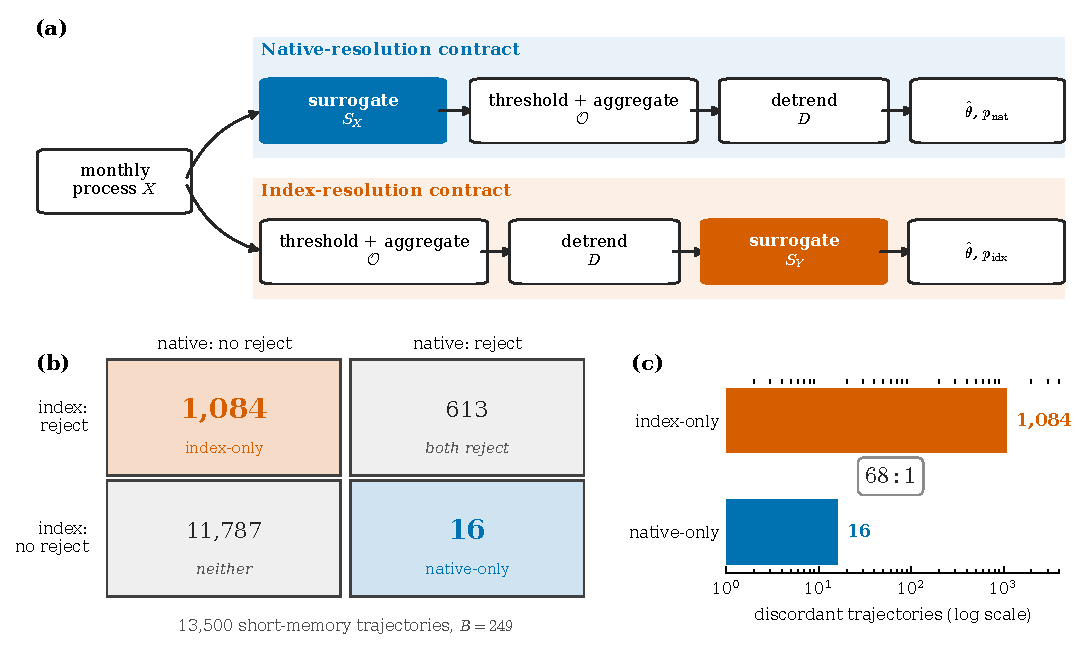
\includegraphics[width=\textwidth]{fig1_null_placement_discordance.pdf}
\caption{\label{fig:nullplacement}Native and index-level contracts act on opposite sides of the transformation pipeline and yield strongly asymmetric paired conclusions. (a) The native surrogate is applied before thresholding, annual aggregation, and detrending; the index-level IAAFT surrogate is applied afterward. In the null-transport formulation, the upper branch estimates a pushed-forward native law $\mathcal P_\#K_X(x,\cdot)$, whereas the lower branch substitutes an aggregate-space kernel $K_Y(\mathcal Px,\cdot)$. (b) Paired outcomes in 13,500 confirmatory short-memory trajectories. (c) Index-only and native-only discordant counts on a logarithmic scale.}
\end{figure}

\subsection{Seasonal event geometry amplified the discrepancy and supplied a mitigation}\label{sec:seasonresults}

The expected annual event count was fixed at three while $\Neff$ decreased from 12 at $\lambda=0$ to approximately 4.96 at $\lambda=4$. Index-only discordance rose from 4.41\% [3.70\%, 5.25\%] under uniform monthly event probability to 16.22\% [14.88\%, 17.66\%] under the strongest concentration, a risk difference of 11.81 percentage points (Fig.~\ref{fig:concentration}). The contrast had the same direction in all nine generator-family $\times\phi$ strata. Across the full grid, index-only discordance was 4.41\%, 4.30\%, 6.19\%, 9.04\%, and 16.22\% for $\lambda=0,0.5,1,2,4$, respectively. The native-resolution rejection rate remained near its benchmark level across the concentration grid.

\begin{figure}[t]
\centering
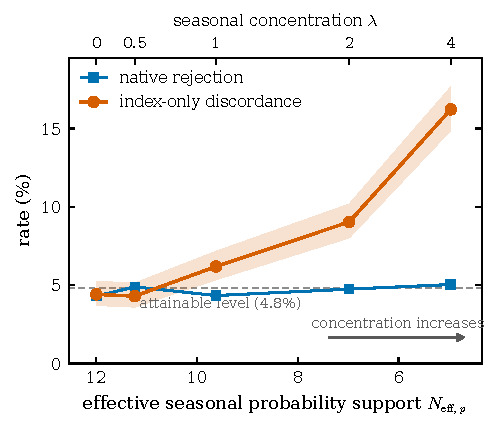
\includegraphics[width=0.62\textwidth]{fig2_seasonal_concentration.pdf}
\caption{\label{fig:concentration}Seasonal concentration amplifies index-only discordance. The expected annual event count remains fixed at three while $\Neff$ decreases as $\lambda$ increases. Index-only discordance rises from 4.41\% under uniform monthly probability to 16.22\% under the strongest concentration; native rejection remains close to its attainable Monte Carlo level. Error band: 95\% Wilson interval.}
\end{figure}

The independent probability-equalization experiment reproduced the concentration effect. Index-only discordance was 15.85\% [14.00\%, 17.90\%] for the concentrated $\lambda=4$ profile and 3.93\% [3.01\%, 5.10\%] for the oracle uniform profile, an absolute reduction of 11.93 percentage points, or about 75\% of the concentrated-profile rate (Fig.~\ref{fig:equalization}). The principal 30-year percentile construction produced 3.48\% [2.63\%, 4.60\%]; 15- and 60-year references produced 3.85\% and 4.00\%. The estimated probability geometry converged toward uniformity with reference length: the RMSE of the true monthly event probabilities relative to 0.25 decreased from 0.102 to 0.075 to 0.053, while $\Neff$ increased from 10.93 to 11.34 to 11.63.

\begin{figure}[t]
\centering
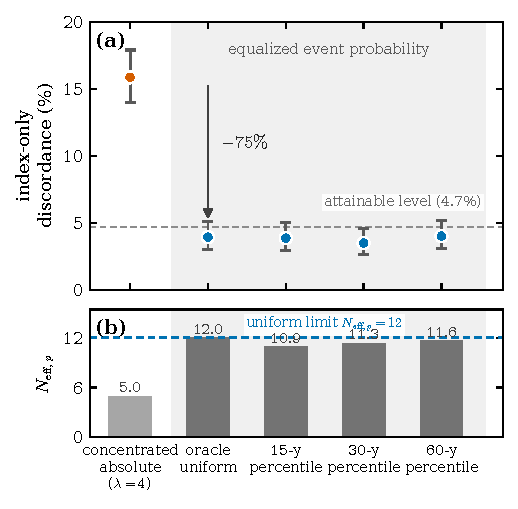
\includegraphics[width=0.62\textwidth]{fig3_probability_equalization.pdf}
\caption{\label{fig:equalization}Seasonal probability equalization substantially reduces concentration-associated discordance in an independent 1350-trajectory experiment. The oracle uniform construction lowers index-only discordance from 15.85\% to 3.93\%; month-specific percentile thresholds estimated from independent 15-, 30-, and 60-year references behave similarly. The lower panel shows the corresponding movement of $\Neff$ toward its uniform limit of 12.}
\end{figure}

These results identify seasonal event geometry as an amplifier, not as the sole source of the discrepancy. The equalized constructions retain a small residual index/native difference, and changing a physical threshold to a percentile threshold changes the scientific event definition as well as its inferential geometry.

\subsection{Gaussian controls localize the discrepancy}\label{sec:ablationresults}

The mechanism-localization controls produced a sharp contrast between continuous linear aggregation and hard threshold counts (Fig.~\ref{fig:ablation}). For the raw annual Gaussian mean, oracle, native, and index-level rejection rates were 5.3\%, 3.7\%, and 4.7\%, respectively; after cubic detrending they were 6.3\%, 4.0\%, and 3.7\%. Thus the large index-only asymmetry was absent for the continuous Gaussian control.

For the hard annual count with uniform monthly event probability ($\lambda=0$), rejection was 7.7\% under both oracle and native nulls and 11.0\% under annual IAAFT; index-only versus native discordance was 4.0\%. Under concentrated event geometry ($\lambda=4$), the separation became large: oracle rejection was 5.3\%, native rejection 3.7\%, and annual IAAFT rejection 23.3\%. There were 59 index-only and zero native-only decisions among 300 trajectories, giving 19.7\% index-only discordance.

The soft-threshold path showed that generic smooth nonlinearity was not enough to reproduce the hard-count effect. At $\lambda=4$, index-level rejection remained between 5.0\% and 7.3\% for $\tau\in\{2,1,0.5,0.25,0.1\}$, while the median ratio of index-null to oracle-null standard deviation of $\widehat\theta$ remained between about 0.87 and 0.92. At the hard-count limit, index rejection rose to 23.3\% and the dispersion ratio fell abruptly to 0.54, whereas the native/oracle dispersion ratio remained 0.98. A smaller near-zero diagnostic showed a progressive transition below $\tau=0.1$, approaching the hard-count behavior rather than a mathematical discontinuity at $\tau=0$ (Supplement).

\begin{figure}[t]
\centering
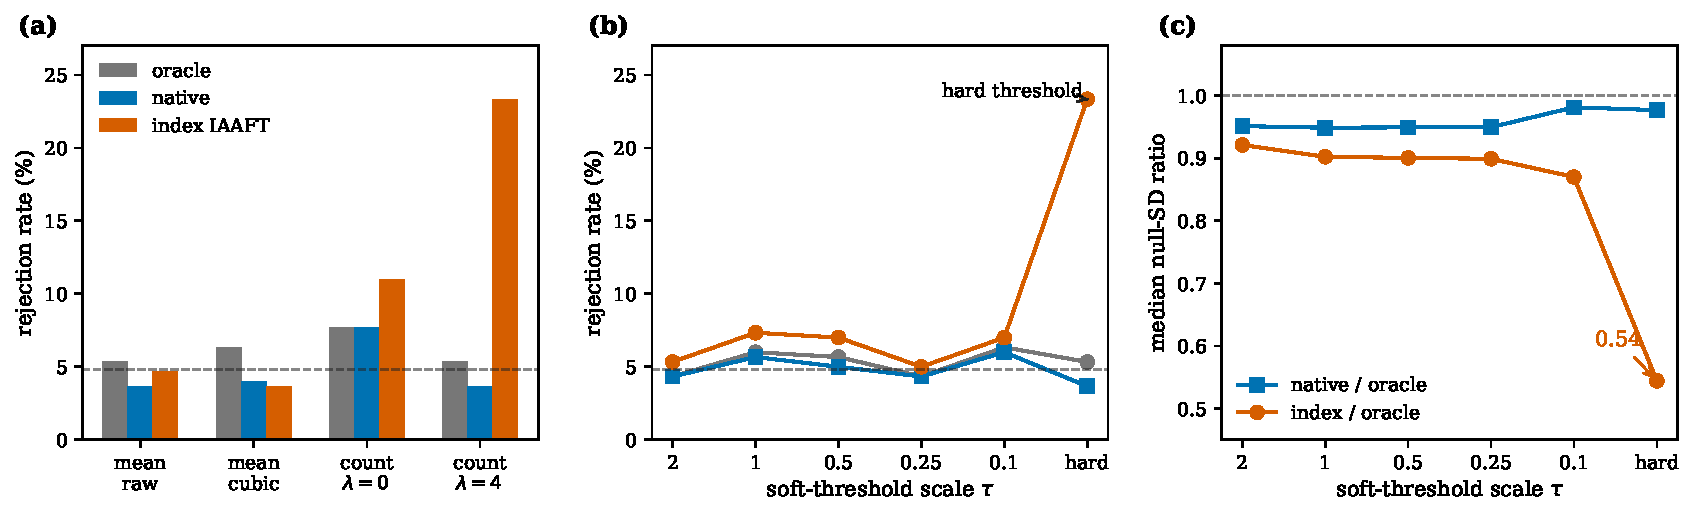
\includegraphics[width=\textwidth]{fig4_gaussian_operator_ablation.pdf}
\caption{\label{fig:ablation}Gaussian oracle and operator-ablation diagnostics. (a) Rejection rates for a continuous annual mean and hard threshold counts, pooled over $\phi=0.2,0.5,0.8$ (100 trajectories each; $B=249$). The large index-level excess is absent for the Gaussian mean and strongest for the concentrated hard count. (b) At $\lambda=4$, rejection remains near the oracle/native range along the soft-threshold path until the observable approaches the hard-count geometry. (c) The median native/oracle null-SD ratio remains near one; the index/oracle ratio falls to 0.54 at the hard count. These analyses were designed after the confirmatory benchmark and are interpreted mechanistically rather than confirmatorily.}
\end{figure}

Additional diagnostics locate the projection through which the lower-tail Ferro--Segers test produces excess rejection relative to the generative/native reference. At the hard-count limit, the annual IAAFT null produced fewer adjacent upper-tail exceedance pairs (median ensemble mean 2.34) than the oracle and native nulls (2.88 and 2.89), a smaller inter-exceedance-gap standard deviation (8.59 versus 9.95 oracle), and a higher mean null extremal-index estimate (0.972 versus 0.892 oracle). Simultaneously, the null standard deviation of $\widehat\theta$ was approximately 0.069 for annual IAAFT versus 0.132 for the oracle. At $\tau=0.1$ these differences were small. The effect was not eliminated by increasing IAAFT from 30 to 100 or 300 iterations, and a global phase-dispersion diagnostic did not show phase collapse. The evidence is therefore more consistent with post-transformation constraint rigidity in the extremal-spacing geometry than with premature algorithm termination or global phase locking.

\subsection{Within-fiber perturbations provide direct numerical evidence against strong lumpability}\label{sec:fiberresults}

The within-fiber construction asks the lumpability question directly: can the native pushed-forward null change when the observed aggregate is held exactly fixed? It can. For every pair, $x$ and $\widetilde x$ had identical threshold indicators at every month, identical annual count sequences, and identical calendar-month value multisets; only the hidden monthly organization of amplitudes, and hence the standardized target spectrum used by the native contract, was altered.

For the Ferro--Segers projection under $\lambda=0$, the median scaled Wasserstein distance between within-fiber native nulls was 0.175, compared with 0.086 between two independent same-$x$ ensembles, a median distance ratio of 1.93. The within-fiber distance exceeded its same-$x$ Monte Carlo baseline in 73.3\% of pairs (one-sided sign-test $p=5.45\times10^{-6}$). Under $\lambda=4$, the median distances were 0.335 versus 0.090, a ratio of 3.31; 91.1\% of fiber distances exceeded baseline ($p=6.92\times10^{-17}$). A two-sample KS comparison distinguished 70.0\% of the $\lambda=4$ within-fiber Ferro--Segers null pairs at the 5\% level, compared with 1.1\% of same-$x$ Monte Carlo controls.

The effect was larger for projections directly sensitive to order and second-order structure. The median within-fiber/same-$x$ distance ratios were 4.55 for lag-one correlation, 15.28 for raw $T_{\rm diff}$, and 3.97 for low-frequency power share under $\lambda=4$ (Fig.~\ref{fig:fiber}). For $T_{\rm diff}$, all 90 within-fiber pairs were distinguished by the KS comparison for both $\lambda=0$ and $\lambda=4$. Under $\lambda=4$, the hidden target-spectrum distance was strongly associated with transported-null distance for $T_{\rm diff}$ (Spearman $\rho\approx0.90$), while the relationship was weaker for Ferro--Segers. This is consistent with the data-processing hierarchy in Eq.~\eqref{eq:dataprocessing}: a kernel-level difference can project strongly onto one statistic and weakly onto another.

\begin{figure}[t]
\centering
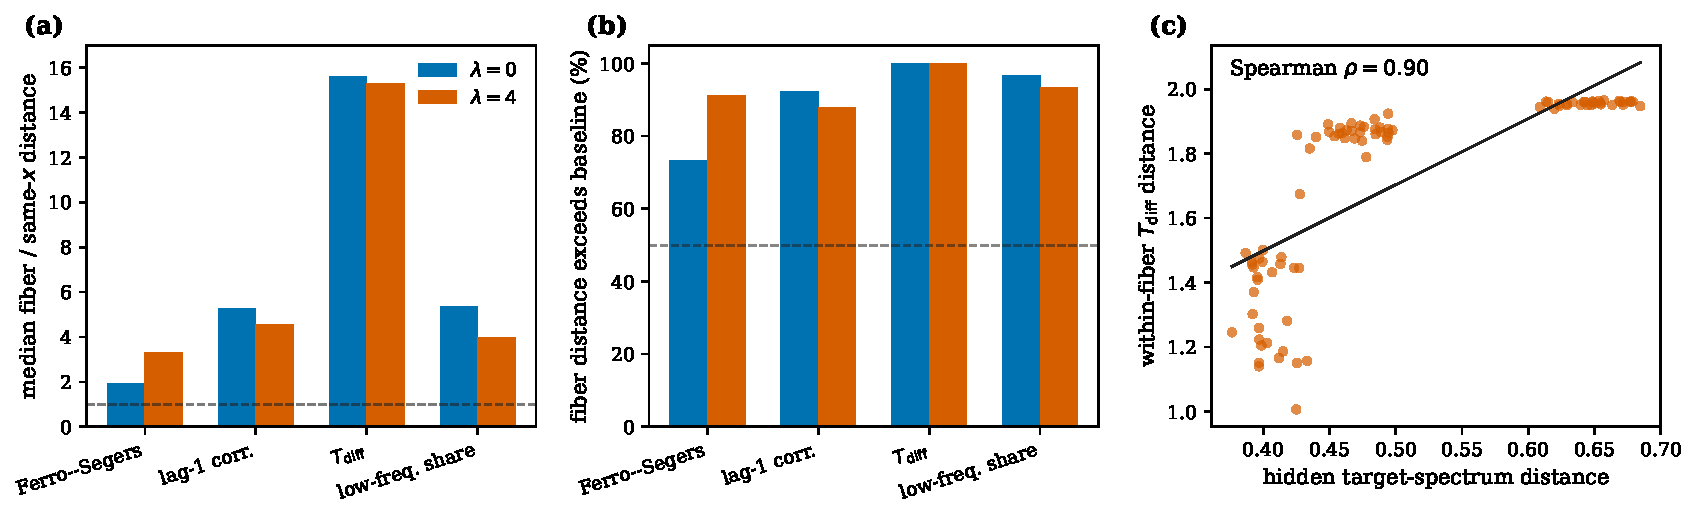
\includegraphics[width=\textwidth]{fig5_within_fiber_lumpability.pdf}
\caption{\label{fig:fiber}Within-fiber evidence against strong lumpability of the implemented native surrogate kernel. (a) Median ratio of within-fiber to same-$x$ Monte Carlo baseline distance for four pushed-forward projections. (b) Fraction of pairs for which the within-fiber distance exceeds the corresponding same-$x$ baseline; the dashed line marks 50\%. (c) For $\lambda=4$, hidden target-spectrum separation is strongly associated with the within-fiber distance of $T_{\rm diff}$ (Spearman $\rho\approx0.90$). The construction preserves the entire monthly threshold-indicator chronology, annual counts, and calendar-month value multisets exactly.}
\end{figure}

The final reject/no-reject decision changed much less often than the full null distributions, which is expected: decision compatibility is weaker than statistic-level or kernel-level compatibility. The within-fiber result therefore should not be read as claiming that every aggregate test must disagree. It establishes the more basic point needed for null transport: $\mathcal O(x)$ does not determine the native pushed-forward null for the implemented contract.

\subsection{The frozen SINCA application shows large applied null-transport distortion}\label{sec:sincaresults}

All 31 frozen stations passed the technical conservation gates. Under the fixed $50\,\mu\mathrm{g\,m^{-3}}$ event threshold, the weekly index-level IAAFT null rejected at all 31 stations, whereas the native daily transported null rejected at two. The paired outcomes were therefore 29 index-only, zero native-only, two both, and zero neither (Table~\ref{tab:sinca}; Fig.~\ref{fig:sinca}). The exact region-level sign-flip test gave $p=0.003906$. After Benjamini--Yekutieli adjustment across the 31 stations, 27 index-level results remained significant and no native-resolution result did.

The projected nulls differed primarily in location rather than through universal narrowing. Across stations, the median observed Ferro--Segers estimate was 0.535, the median native-null center was 0.557, and the median index-null center was 0.993. Thus the median center gap
\[
G_s=\operatorname{median}(\widehat\theta^\star_{\rm index,s})-\operatorname{median}(\widehat\theta^\star_{\rm native,s})
\]
was 0.422. By contrast, the median null-width ratio was 1.120. The prespecified width-contraction mechanism was not supported: the Spearman association between frozen $\Neff$ and $\log R_s$ was $\rho=-0.379$, with region-cluster bootstrap 95\% interval $[-0.624,0.136]$. The point estimate is opposite the predicted direction and the interval includes zero. The applied result therefore refines the synthetic mechanism interpretation: null transport can fail through a displacement of the full statistic distribution, not necessarily through under-dispersion.

\begin{table}[t]
\centering
\caption{Prospectively frozen SINCA PM$_{2.5}$ application. Station-level rejection uses strict Monte Carlo $p<0.05$ with $B=499$ and Ferro--Segers $q=0.90$.}\label{tab:sinca}
\small
\setlength{\tabcolsep}{4pt}
\begin{tabular}{lrrrrrr}
\toprule
Threshold branch & Idx rej. & Nat. rej. & Idx-only & Nat.-only & Both & Neither\\
\midrule
Fixed $50\,\mu$g m$^{-3}$ & 31 & 2 & 29 & 0 & 2 & 0\\
Probability equalized & 6 & 1 & 5 & 0 & 1 & 25\\
\bottomrule
\end{tabular}
\normalsize
\end{table}

Probability equalization sharply reduced the discrepancy. Realized $\Neff$ moved to approximately 12 at each station; index-level rejection fell from 31 to six stations, native rejection changed from two to one, and index-only discordance fell from 29 to five. The region sign-flip result weakened to $p=0.0625$, and no station remained significant after BY adjustment under either contract. The median center gap fell from 0.422 to 0.097 and decreased in all 31 stations; the index-level $p$-value increased in 30 of 31 stations. This paired intervention is stronger evidence for the role of seasonal event geometry than a cross-sectional association alone.

\begin{figure}[t]
\centering
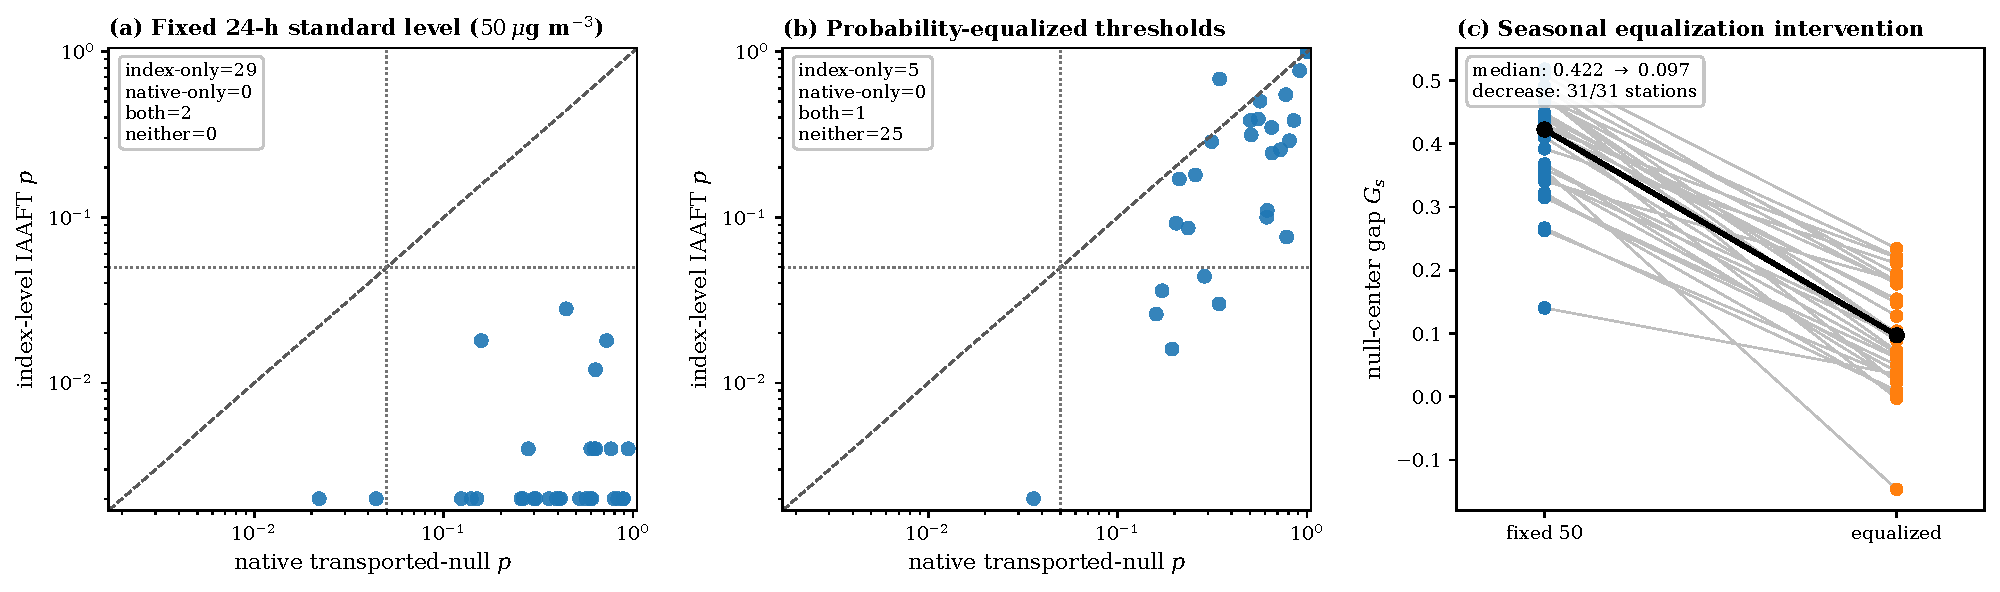
\includegraphics[width=\textwidth]{fig6_sinca_application.pdf}
\caption{\label{fig:sinca}Prospectively frozen SINCA PM$_{2.5}$ application. (a) Native transported-null versus weekly index-level IAAFT $p$-values under the fixed $50\,\mu\mathrm{g\,m^{-3}}$ event threshold. Dotted lines mark 0.05 and the dashed line marks equality. (b) The same comparison after month-specific probability equalization. (c) Station-level index-minus-native Ferro--Segers null-center gap $G_s$ before and after equalization; gray lines join the same station and the black line joins the medians. The center gap decreases in all 31 stations.}
\end{figure}

The prespecified sensitivities confirmed that the magnitude of the transport defect is statistic-dependent. At $q=0.85$, the fixed-threshold branch rejected at 31/31 stations under the index null and 10/31 under the native null; after probability equalization the counts were 2/31 and 0/31. For normalized $T_{\rm diff}$, the corresponding fixed-threshold counts were only 4/31 and 1/31, with 5/31 and 2/31 after equalization. The exposure-standardized missingness sensitivity was technically defined at 22 stations; all 22 rejected under the index-level null, one rejected under the native null, giving 21 index-only and one both. Thus neither the particular missing-day expectation fill nor a single choice of Ferro--Segers quantile explains the primary applied asymmetry, while the weaker $T_{\rm diff}$ contrast illustrates the statistic-projection hierarchy in Eqs.~\eqref{eq:dataprocessing}--\eqref{eq:decisionbound}.

\section{Discussion}\label{sec:discussion}

\subsection{The central problem is null transport, not merely null placement}\label{sec:discussiontransport}

The original empirical observation motivating this study was that moving a surrogate constraint from native resolution to a threshold-derived annual index changed the conclusion. The kernel formulation shows why the deeper question is not simply location. The native procedure defines a transported law $L_x=\mathcal G_\#K_X(x,\cdot)$. An aggregate-space surrogate can represent the same inferential contract only if an appropriate quotient or model-dependent transported law exists and the chosen aggregate kernel matches it.

Strong $\mathcal G$-lumpability is the clean case: all native microstates in the same fiber generate the same pushed-forward null. Proposition~\ref{prop:quotient} then yields a unique quotient kernel. When lumpability fails, Proposition~\ref{prop:halfdiam} shows that no null using only the aggregate can be uniformly exact over the fiber. Additional assumptions about unresolved microstates are required, as in Eq.~\eqref{eq:modeltransport}. This is an identifiability statement about the null contract, not a claim that aggregate-level inference is impossible or that the native contract is universally preferable.

The within-fiber experiment provides direct numerical evidence that the implemented native marginal-and-spectrum contract is not strongly lumpable with respect to the threshold-and-count map. The two fiber mates preserve substantially more than the annual count: the complete event chronology and each calendar-month amplitude multiset are identical. Yet changing hidden amplitude organization changes the monthly spectral target and, downstream, the annual null distribution. The aggregate therefore erases information that remains active in the native randomization rule.

\subsection{What the mechanism-localization controls identify}\label{sec:discussionmechanism}

The Gaussian controls substantially narrow the mechanism. Annual IAAFT does not show a comparable excess rejection for a continuous linearly aggregated Gaussian observable. The effect grows as the observation approaches a hard threshold count, and under concentrated synthetic event geometry the annual IAAFT null becomes both shifted toward $\widehat\theta=1$ and strongly under-dispersed relative to the oracle/native null. The lower-tail test consequently rejects more often.

The SINCA application shows why this mechanism should be stated at the level of the \emph{full projected null distribution}, not as a universal claim of null contraction. With the fixed PM$_{2.5}$ threshold, the weekly index null was again displaced sharply toward $\widehat\theta=1$, but its median standard deviation was slightly larger, not smaller, than that of the native transported null. The prespecified width-contraction association with $\Neff$ was not supported. What replicates across synthetic and observational settings is therefore the distributional distortion induced by imposing marginal-and-spectrum constraints after a lossy threshold-and-aggregation map; the distortion may appear in the center, width, tails, or combinations of these features.

The evidence is consistent with a mechanism of \emph{post-transformation constraint rigidity}. Hard thresholding and aggregation map many distinct native amplitude configurations to the same or nearby count geometry. Applying IAAFT after that reduction simultaneously fixes the exact transformed sample marginal and approximately fixes the transformed sample spectrum. In the synthetic hard-count setting, this regularizes upper-rank spacing and narrows the Ferro--Segers null; in SINCA, the dominant signature is a much larger upward displacement of the null center. Imposing the spectral constraint at native resolution and only then applying the threshold-count map leaves a different family of admissible event arrangements. Constraint rigidity is therefore a structural mechanism for null-transport distortion, while the exact projected manifestation is statistic- and data-dependent.

This interpretation is more specific than a generic criticism that Fourier surrogates condition on an estimated spectrum. That issue is well known in the surrogate literature \cite{SchreiberSchmitz2000,Kugiumtzis1999}. Here both contracts are spectrally constrained; what differs is the side of a lossy transformation on which the constraint is imposed. The exactly solvable counterexample demonstrates that marginal preservation plus microstate spectral conditioning can destroy lumpability under aggregation, and the Gaussian/within-fiber diagnostics show the same structural signature in the implemented contracts. We do not claim that spectral-error magnitude itself is the causal mediator. Across the soft-threshold path, increasing spectral mismatch and null contraction move together, but within a fixed $\tau$ the relationship is much weaker. They are better viewed as parallel manifestations of increasing constraint rigidity.

\subsection{Seasonal probability geometry controls severity, not existence}\label{sec:discussionseason}

Lemma~\ref{lem:copula} explains why seasonal event probability is a natural intervention coordinate. Conditional on the temporal copula, changing the threshold construction acts through $\mathbf p$. Concentrating a fixed expected annual event count reduces $\Neff$ and substantially increases decision-level discordance. Probability equalization reverses most of that increase in an independent cohort.

The prospectively frozen SINCA application provides an observational counterpart. With the fixed $50\,\mu\mathrm{g\,m^{-3}}$ level, the 31 stations had $\Neff$ between 3.40 and 5.67 and showed 29 index-only decisions. Equalizing monthly event probabilities moved $\Neff$ close to 12, reduced index-only decisions to five, and reduced the index-minus-native null-center gap at every station. Because the intervention changes the event definition, it is not a regulatory recommendation; its role is mechanistic. The fixed standard level remains the primary scientific event.

The new controls refine the interpretation. Hard threshold-count geometry produces some vulnerability even under uniform $\mathbf p$, while strong seasonal concentration magnifies it. Thus $\Neff$ should be treated as an amplifier of the null-transport problem rather than its universal cause. The Gaussian covariance formula in Proposition~\ref{prop:gausscov} also makes clear that $\Neff$ alone cannot determine the annual dependence law: the full vector $\mathbf p$ and the native correlation structure both enter $\gamma_C(k)$.

Month-specific percentile thresholds are therefore a statistically meaningful mitigation when a seasonally relative event definition is scientifically acceptable, but they are not a generic repair. A common physical threshold and a percentile threshold define different events. The event definition should not be changed solely to make a surrogate test more favorable.

\subsection{Implications for surrogate and resampling inference}\label{sec:broader}

The framework is not restricted to IAAFT or to climate extremes and air-pollution indices. Any workflow that applies a randomization, permutation, bootstrap, or conditional null after a lossy deterministic transformation faces the same structural question: is the post-transformation null the pushforward of the intended native contract, and if not, what information was lost? Lumpability provides a sharp existence criterion for an aggregate-only quotient kernel, while the statistic-level data-processing inequality clarifies why some diagnostics can remain stable even when the underlying kernels differ.

This perspective also separates validity from scientific interpretation. An index-level surrogate can be perfectly coherent for a hypothesis defined solely on the index, even if it is not a transported native null. The error occurs only when rejection of that index-level contract is interpreted as evidence against a native-resolution mechanism that the aggregate null does not represent. Conversely, a native-resolution non-rejection cannot establish absence of organization unless the native contract has demonstrated sensitivity to scientifically relevant alternatives.

\subsection{Limitations}\label{sec:limitations}

Several limitations bound the claims. First, the large computational discrepancy is demonstrated for a particular pair of marginal-and-spectrum surrogate contracts, with IAAFT at aggregate resolution and a calendar-group constrained spectral surrogate at native resolution. The theory is general, but empirical magnitudes are algorithm- and statistic-specific. Second, the analytical counterexample proves a structural possibility for a simplified spectral-tilted permutation kernel, not for IAAFT itself; the implemented contracts are assessed numerically through Gaussian and within-fiber diagnostics. Third, the original confirmatory benchmark fixed cubic detrending. The later Gaussian control indicates that detrending alone is not the dominant source of the synthetic discrepancy, but deterministic residualization changes covariance structure and should not be considered innocuous in all settings. Fourth, the Gaussian mechanism-localization and within-fiber analyses were designed after inspection of the confirmatory synthetic result; they are diagnostic evidence rather than independent confirmatory replication.

The SINCA analysis addresses that last limitation only partially. Its 31-station cohort and inferential protocol were frozen before any application-level surrogate output was inspected, but the application itself was designed after the theoretical and synthetic findings were known. It is therefore a prospective applied validation of predicted qualitative behavior, not a blinded replication of the entire research program. The eight-year window trades historical depth for recent data quality and stable coverage, and the station network is observational rather than a probability sample of Chilean exposure. Region-level sign-flip inference reduces but does not eliminate spatial dependence concerns. The daily $50\,\mu\mathrm{g\,m^{-3}}$ event uses the level of Chile's 24-hour primary standard, while statutory exceedance is defined using the annual 98th percentile; our station-day event should not be interpreted as a legal noncompliance indicator. Finally, Ferro--Segers has finite-sample and tie-related behavior for count-derived observables. The weaker $T_{\rm diff}$ contrast in SINCA and the stronger within-fiber $T_{\rm diff}$ contrast in simulation together reinforce that transport defects are projected differently by different statistics.

\subsection{Practical recommendations}\label{sec:recommendations}

Four practices follow. First, state explicitly the resolution at which a surrogate or resampling constraint is defined and whether the scientific hypothesis concerns the native process or only the derived index. Second, when a native interpretation is intended, examine whether the required null can be transported through the preprocessing map; a within-fiber diagnostic is a practical way to detect hidden dependence on information lost by the aggregate. Third, for threshold-derived indices, report the seasonal event-probability vector or a concentration summary such as $\Neff$, and consider seasonally relative thresholds only when they are scientifically defensible. Fourth, distinguish null calibration from power: non-rejection under a highly constrained native contract does not support absence claims without sensitivity analysis against relevant alternatives.

The broader lesson is that coarse-graining changes not only the data but potentially the hypothesis that a randomization procedure represents. The correct inferential object is therefore the transported null, not an automatically substituted null chosen only because it is convenient at the resolution of the final index.

\section{Reproducibility statement}\label{sec:reproducibility}

The original synthetic benchmark and probability-equalization analyses were executed under sequentially fixed protocols with deterministic seed namespaces, archived code hashes, technical conservation gates, and an independently written audit implementation. The later Gaussian-control, operator-ablation, near-zero, extremal-spacing, and within-fiber analyses were designed as mechanism diagnostics after the confirmatory results and use separate deterministic seed namespaces. The within-fiber construction includes explicit checks for identical threshold-indicator chronology, annual counts, and calendar-month value multisets.

For SINCA, the 31-station cohort was frozen before surrogate computation; the station-list SHA-256 is recorded in the Supplement and protocol manifest. The missingness rule, weekly aggregation, preprocessing design, native and index surrogate contracts, $B=499$, cross-station inference, multiplicity adjustment, probability-equalization branch, and sensitivity statistics were all written to a versioned inferential protocol before the primary station-level surrogate outputs were inspected. Native-surrogate gates verified exact calendar-month value-multiset and threshold-count preservation. The companion reproducibility package contains the frozen cohort, protocol manifest, analysis-ready PM$_{2.5}$ extract, executable scripts, station-level outputs, and sensitivity results.


\section*{Acknowledgements}
OpenAI ChatGPT (GPT-5.6 Sol) was used to assist with manuscript revision. The author specified the scientific questions and analysis designs, reviewed the generated text and code, inspected the numerical outputs, and assumes full responsibility for the content. The author reports no external funding for this work.

\paragraph{Data and code availability.}
The complete reproducibility package corresponding to this manuscript is maintained through the versioned Zenodo archive associated with the public GitHub repository \texttt{mauricio-herrera/null-placement-surrogate-inference}. Release v2.0.0 contains the original confirmatory synthetic outputs, null-transport theory diagnostics, Gaussian and within-fiber analyses, the prospectively frozen SINCA station cohort and inferential protocol, the analysis-ready 2018--2025 PM$_{2.5}$ extract used here, executable scripts, and station-level outputs. Source air-quality observations are publicly available from Chile's National Air Quality Information System (SINCA) and were retrieved through the AtmChile interface.

\section*{Conflict of Interest}
The author declares no conflict of interest.

\input{references_final.bbl}

\end{document}
